%  The AAU Poster Theme.
%  2013-05-08 v. 1.1.0
%  Copyright 2013 by Jesper Kjær Nielsen <jkn@es.aau.dk>
%
%  This is free software: you can redistribute it and/or modify
%  it under the terms of the GNU General Public License as published by
%  the Free Software Foundation, either version 3 of the License, or
%  (at your option) any later version.
%
%  This is distributed in the hope that it will be useful,
%  but WITHOUT ANY WARRANTY; without even the implied warranty of
%  MERCHANTABILITY or FITNESS FOR A PARTICULAR PURPOSE.  See the
%  GNU General Public License for more details.
%
%  You can find the GNU General Public License at <http://www.gnu.org/licenses/>.
\documentclass[a0paper,portrait]{baposter}
\usepackage{relsize}	
\usepackage{blindtext}
\usepackage[utf8]{inputenc}
\usepackage{sidecap}
% Make latex understand and use the typographic
% rules of the language used in the document.
\usepackage[english]{babel}
% Use the vector font Latin Modern which is going
% to be the default font in latex in the future.
\usepackage{helvet}
% Change the default font family from roman to sans serif
\renewcommand{\familydefault}{\sfdefault} % for text
\usepackage[helvet]{sfmath} % for math
% Choose the font encoding
\usepackage[T1]{fontenc}

%%%%%%%%%%%%%%%%%%%%%%%%%%%%%%%%%%%%%%%%%%%%%%%%
% Graphics and Tables
% http://en.wikibooks.org/wiki/LaTeX/Importing_Graphics
% http://en.wikibooks.org/wiki/LaTeX/Tables
% http://pgfplots.sourceforge.net/
%%%%%%%%%%%%%%%%%%%%%%%%%%%%%%%%%%%%%%%%%%%%%%%%
% You cannot use floats in the baposter theme.
% We therefore load the caption package which provides
% the command \captionof
% Set up how figure and table captions are displayed

\usepackage{caption}
\captionsetup{
	font=small,% set font size to footnotesize
	labelfont=bf % bold label (e.g., Figure 3.2) font
}
% Make the standard latex tables look so much better
\usepackage{array,booktabs}
% For creating beautiful plots
\usepackage{pgfplots}

%%%%%%%%%%%%%%%%%%%%%%%%%%%%%%%%%%%%%%%%%%%%%%%%
% Mathematics
% http://en.wikibooks.org/wiki/LaTeX/Mathematics
%%%%%%%%%%%%%%%%%%%%%%%%%%%%%%%%%%%%%%%%%%%%%%%%
% Defines new environments such as equation,
% align and split 
\usepackage{amsmath}
% Adds new math symbols
\usepackage{amssymb}

%%%%%%%%%%%%%%%%%%%%%%%%%%%%%%%%%%%%%%%%%%%%%%%%
% Colours
% http://en.wikibooks.org/wiki/LaTeX/Colors
%%%%%%%%%%%%%%%%%%%%%%%%%%%%%%%%%%%%%%%%%%%%%%%%
\selectcolormodel{RGB}
% define the three aau colors
\definecolor{aaublue1}{RGB}{33,26,82}% dark blue
\definecolor{aaublue2}{RGB}{113,109,143} % light blue
\definecolor{aaublue3}{RGB}{194,193,204} % lighter blue
\definecolor{luered}{RGB}{147,57,73} % lueneburg red
\definecolor{upbblue}{RGB}{33,26,82}% not yet the right blue
\definecolor{skyblue}{rgb}{0.53, 0.81, 0.92}
\definecolor{orangew}{rgb}{1.0, 0.65, 0.0}
\definecolor{deepskyblue}{rgb}{0.0, 0.75, 1.0}
\definecolor{orangec}{rgb}{1.0, 0.5, 0.0}

\usetikzlibrary{decorations.pathmorphing,calc,shapes,arrows,shapes.geometric,patterns,shadows,arrows.meta,fadings}


%%%%%%%%%%%%%%%%%%%%%%%%%%%%%%%%%%%%%%%%%%%%%%%%
% Lists
% http://en.wikibooks.org/wiki/LaTeX/List_Structures
%%%%%%%%%%%%%%%%%%%%%%%%%%%%%%%%%%%%%%%%%%%%%%%%
% Easier configuration of lists
\usepackage{enumitem}
%configure itemize
\setlist{%
	topsep=0pt,% set space before and after list
	noitemsep,% remove space between items
	labelindent=\parindent,% set the label indentation to the paragraph indentation
	leftmargin=*,% remove the left margin
	font=\color{aaublue1}\normalfont, %set the colour of all bullets, numbers and descriptions to aaublue1
}
% use set<itemize,enumerate,description> if you have an older latex distribution
\setitemize[1]{label={\raise1.25pt\hbox{$\blacktriangleright$}}}
\setitemize[2]{label={\scriptsize\raise1.25pt\hbox{$\blacktriangleright$}}}
\setitemize[3]{label={\raise1.25pt\hbox{$\star$}}}
\setitemize[4]{label={-}}


%%%%%%%%%%%%%%%%%%%%%%%%%%%%%%%%%%%%%%%%%%%%%%%%
% Misc
%%%%%%%%%%%%%%%%%%%%%%%%%%%%%%%%%%%%%%%%%%%%%%%%
% change/remove some names
\addto{\captionsenglish}{
	%remove the title of the bibliograhpy
	\renewcommand{\refname}{\vspace{-0.7em}}
	%change Figure to Fig. in figure captions
	\renewcommand{\figurename}{Fig.}
}
% create links
\usepackage{url}
%note that the hyperref package is currently incompatible with the baposter class

%%%%%%%%%%%%%%%%%%%%%%%%%%%%%%%%%%%%%%%%%%%%%%%%
% Macros
%%%%%%%%%%%%%%%%%%%%%%%%%%%%%%%%%%%%%%%%%%%%%%%%
\newcommand{\alert}[1]{{\color{aaublue1}#1}}


%%%%%%%%%%%%%%%%%%%%%%%%%%%%%%%%%%%%%%%%%%%%%%%%
% Document Start 
%%%%%%%%%%%%%%%%%%%%%%%%%%%%%%%%%%%%%%%%%%%%%%%%
\begin{document}
	%%%%%%%%%%%%%%%%%%%%%%%%%%%%%%%%%%%%%%%%%%%%%%%%
	% Some changes that cannot be made in the preamble
	%%%%%%%%%%%%%%%%%%%%%%%%%%%%%%%%%%%%%%%%%%%%%%%%
	% set the background of the poster
	\background{
		\begin{tikzpicture}[remember picture,overlay]%
		%the poster background color
		\fill[fill=aaublue3] (current page.north west) rectangle (current page.south east);
		%the header
		\fill [fill=aaublue1](current page.north west) rectangle ([yshift=-\headerheight] current page.north east); 
		%\shade[left color=red!80, right color=blue]
		
		\end{tikzpicture}
	}
	
	%%%%%%%%%%%%%%%%%%%%%%%%%%%%%%%%%%%%%%%%%%%%%%%%
	% General poster setup
	%%%%%%%%%%%%%%%%%%%%%%%%%%%%%%%%%%%%%%%%%%%%%%%%
	\begin{poster}{
			%general options for the poster
			grid=false,
			columns=3,
			%  colspacing=4.2mm,
			headerheight=0.1\textheight,
			background=user,
			%  bgColorOne=red!42, %is used when background != user and none
			%  bgColortwo=green!42, %is used when background is shaded
			eyecatcher=true,
			%posterbox options
			headerborder=closed,
			borderColor=aaublue1,
			headershape=rectangle,
			headershade=plain, %shade-lr
			headerColorOne=aaublue1,
			%  headerColorTwo=yellow!42, %is used when the header background is shaded
			textborder=rectangle,
			boxshade=plain,
			boxColorOne=white,
			%  boxColorTwo=cyan!42,%is used when the text background is shaded
			headerFontColor=white,
			headerfont=\Large\sf\bf,
			linewidth=1pt
		}
		%the Eye Catcher (the logo on the left)
		{
			\vspace*{-1cm} 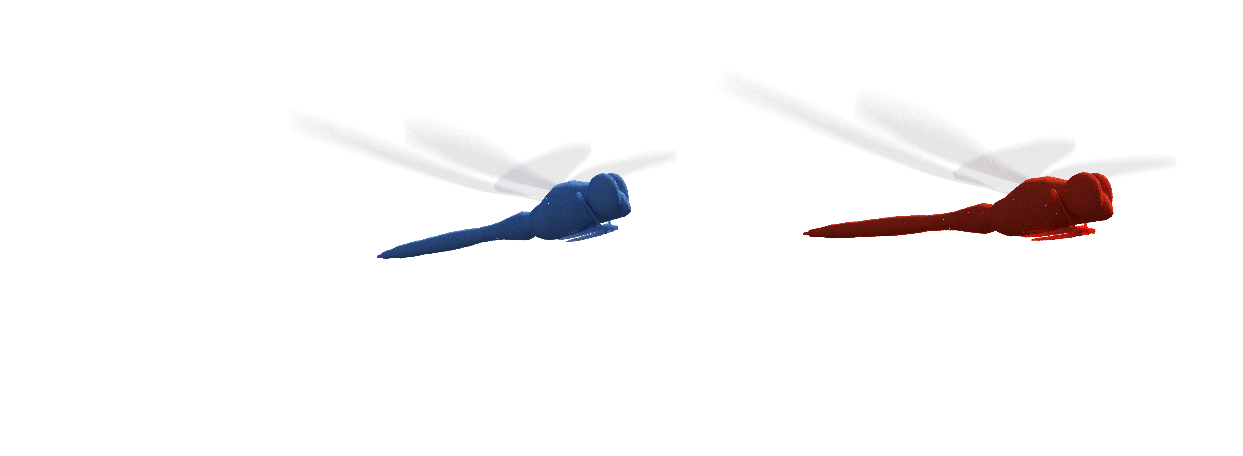
\includegraphics[height=.9\headerheight]{UPB_Logo_WEISS_12_libellen2.pdf}
		}
		%the poster title
		{\color{white}\bf\smaller
			Sphere in a Box: \\ 
			Psychophysical experiments in \\ reality close context
		}
		%the author(s)
		{\color{white}\small
			\vspace*{-0.2cm}
			\vspace{1em}Kai Biermeier, Robin Nagel, Dennis Meier, Philip Schonlau\\
			{\smaller kaibm@mail.upb.de, rnagel@mail.upb.de, , jps96@mail.upb.de}
			
		}
		
		
		%%%%%%%%%%%%%%%%%%%%%%%%%%%%%%%%%%%%%%%%%%%%%%%%
		% the actual content of the poster begins here
		%%%%%%%%%%%%%%%%%%%%%%%%%%%%%%%%%%%%%%%%%%%%%%%%
		
		\begin{posterbox}[name=intro,span=2,column=0,row=0]{Introduction}
			\begin{tabular}{p{0.63\textwidth} p{0.3\textwidth}}
				Psychophysical experiments are designed to provide highly precise parameter estimations. Thus, numerous highly controlled trials are needed in an isolated environment. But due to this isolation the experiment is not completely applicable to reality, because in a native environment there are many confounding variables and a more complex visual stimulus.
				So our approach to get more reality close results is to embed the experiment in a game-engine created surrounding with Unreal4.
				& 
				\vspace{-5pt}
				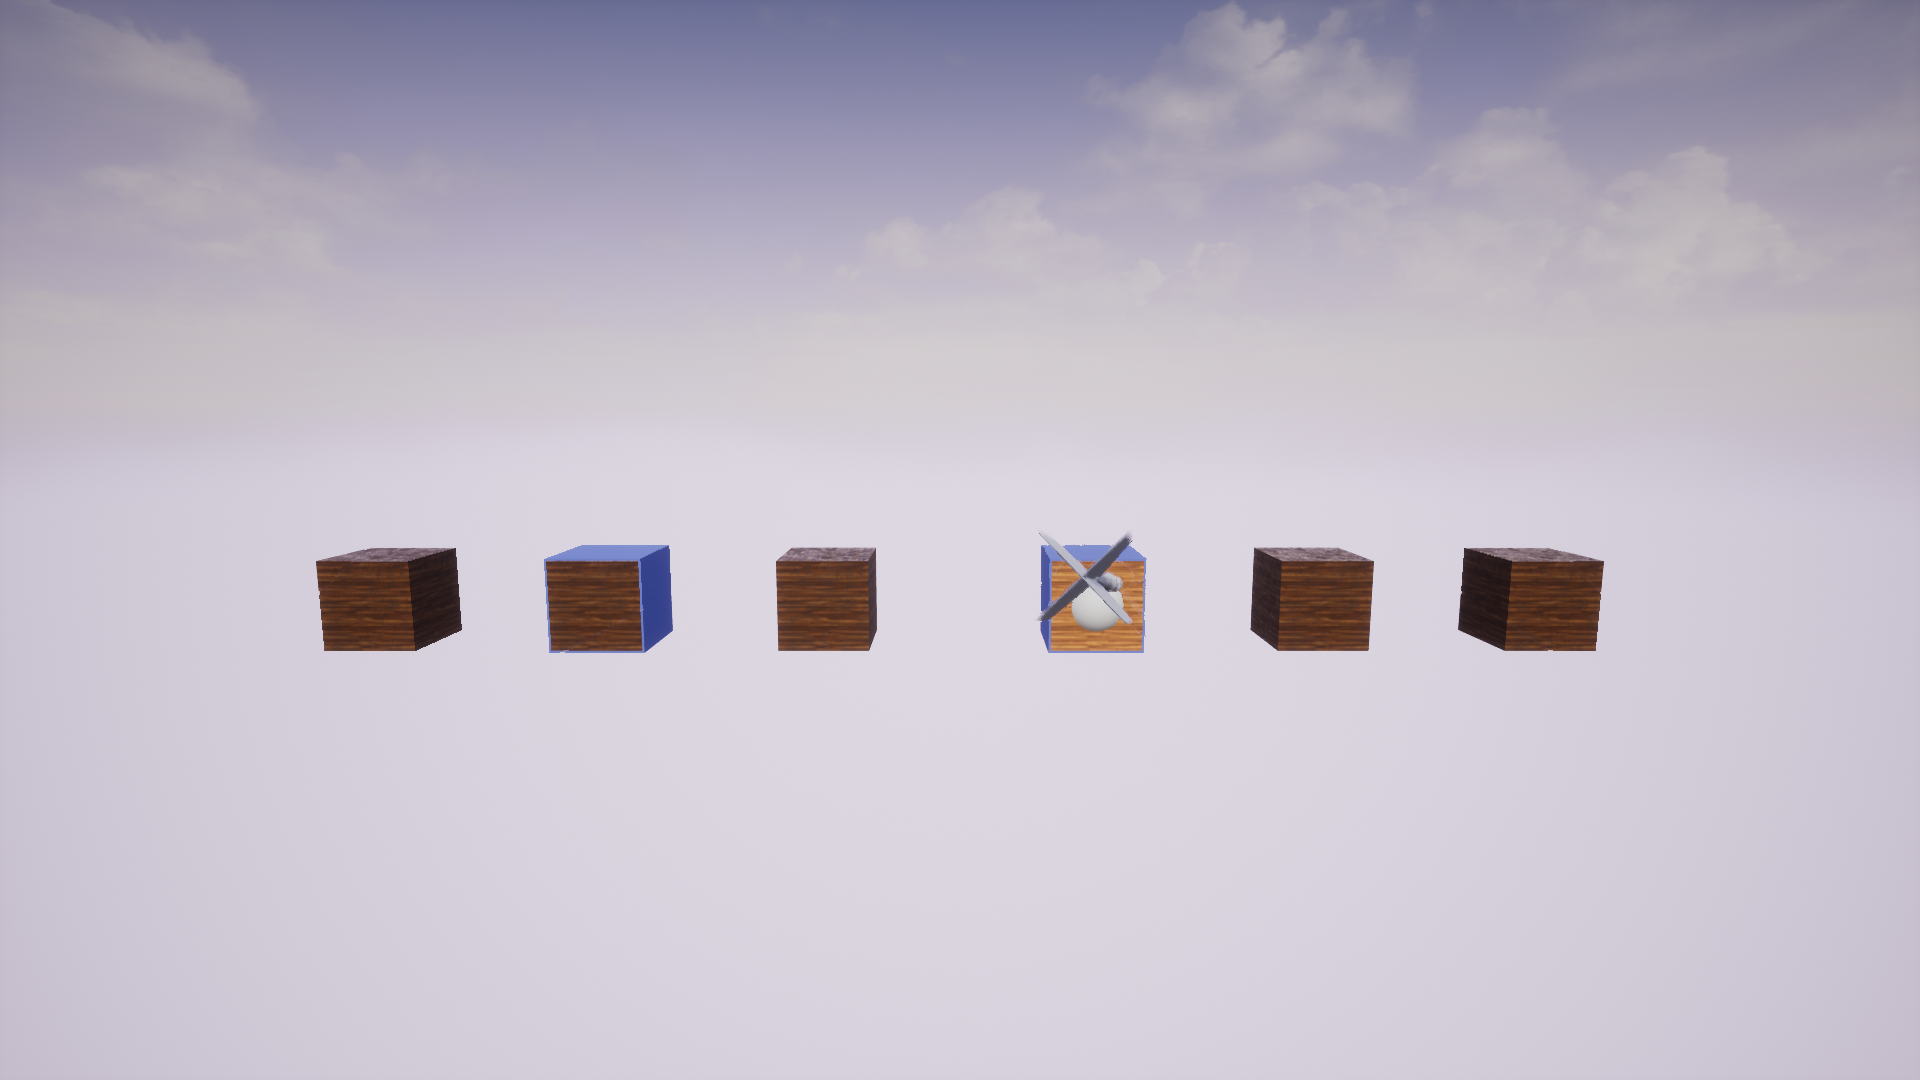
\includegraphics[width=0.32\textwidth]{Screenshots/playerDecision.png}\\
			\end{tabular}
			
		\end{posterbox}
		
		\begin{posterbox}[name=theory,column=0,row=1,below=intro]{Theory}
			\vspace{10pt}
			Visual attention is a complex process. Many stimuli compete for attention resources . Due to limited capacity misjudgments can occur.\\ The experiment focuses on these misjudgments in which we expect one stimuli to get an advantage over the others through a visual contrast. We refer here to Wolfe, J. M., \& Horowitz, T. S. (2004), who show that it is highly propabal that color is important for attention.\\
			 We also obtain to Donk und Soesmann (2011). They show that time is an important variable in order to create effective saliet stimulie especially also in temporal-order-judgement-experiments. To combine time and color predictions we point to Dombrowe, Olivers und Donk (2010).\\ According to Krüger et al. (2016) Bundesen's (1998) theory of visual attention can be applied to temporal-order judgments. Therefore we measure in the experiment associated game the attentional weight w and C the overall processing rate to analyze the relation of time, color and salienz in reality close context.\\
			 We expect the impact of 50 and 400 ms to be lower than the impact of 100ms and 400ms delay, because the to short or to long distance to the stimulus.
			 \vspace{18pt}
		\end{posterbox}
		
		\begin{posterbox}[name=game,span=1,column=1,row=1,below=intro]{Game}
			\begin{itemize}
				\item Multiple boxes are shown on screen.
			\end{itemize}
			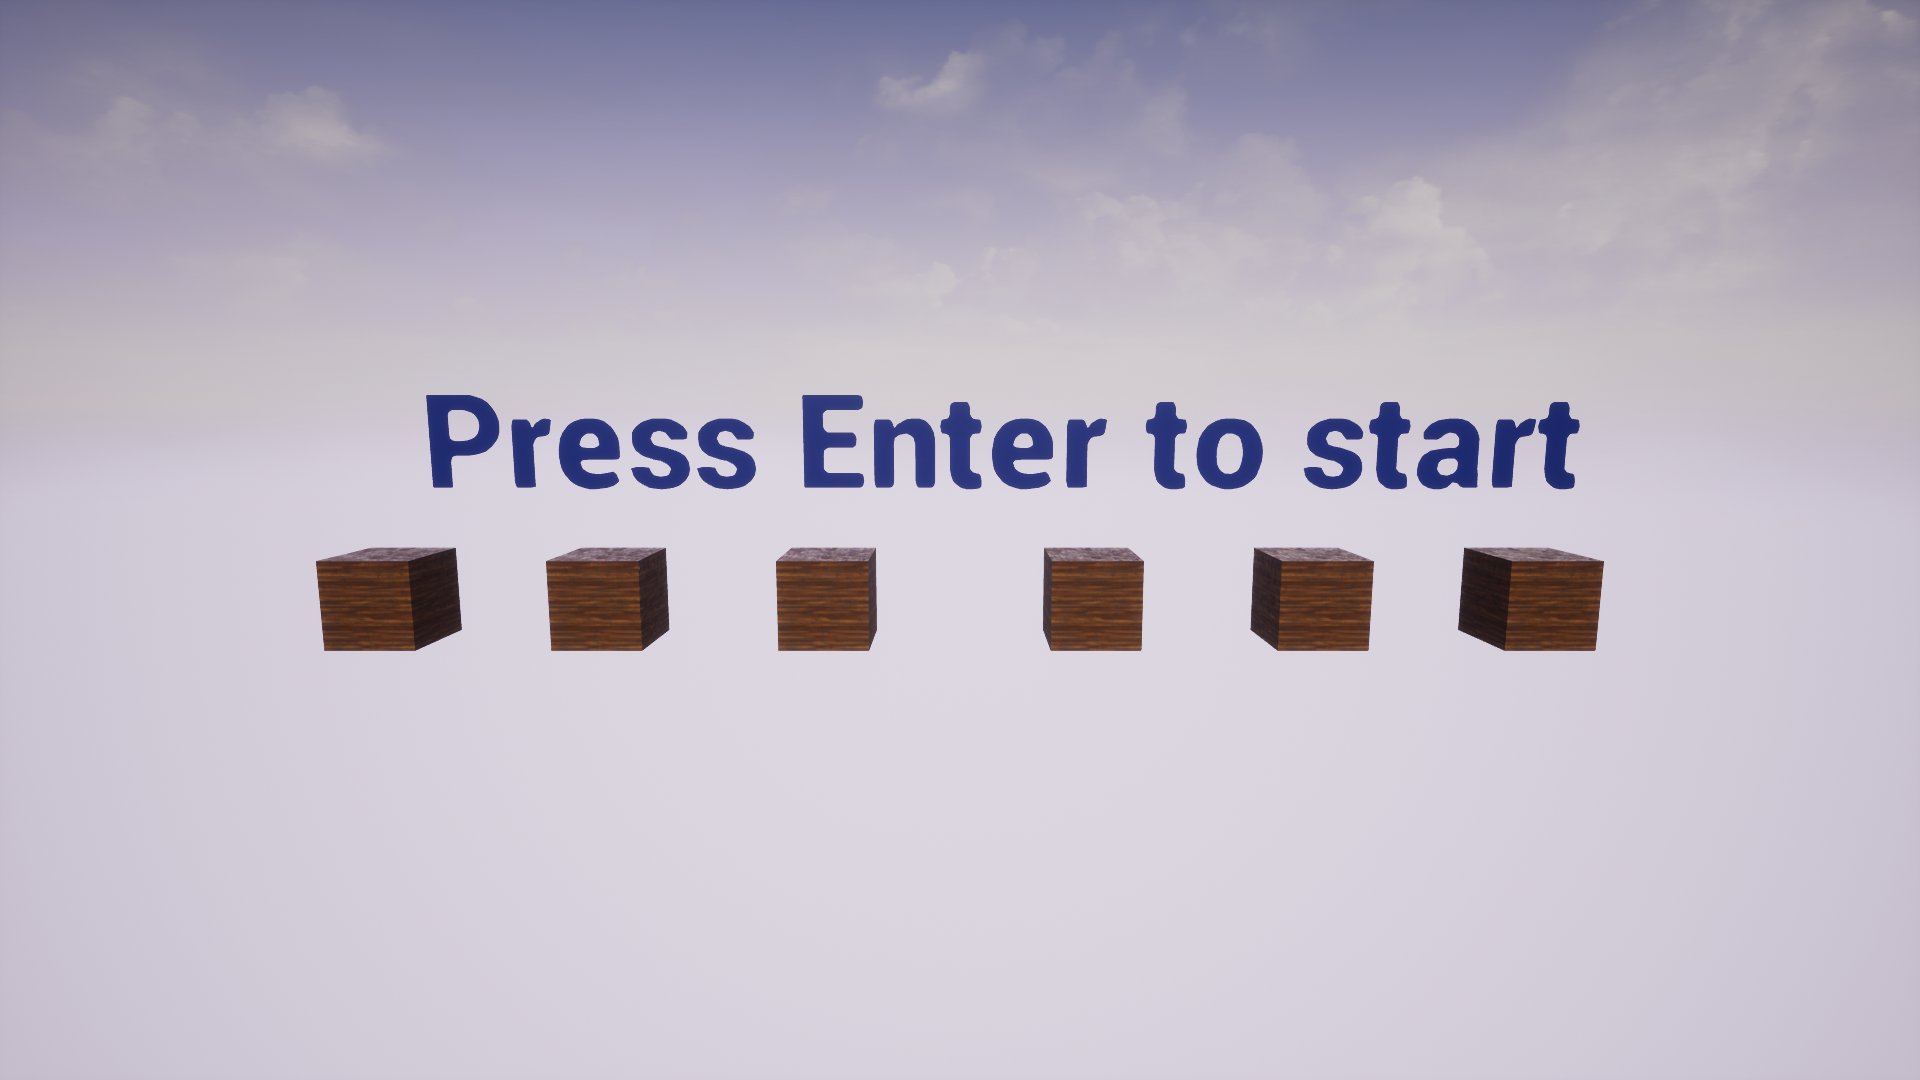
\includegraphics[width=1\textwidth]{Screenshots/gameStart.png}
			\begin{itemize}
				\item Each turn two boxes get selected, one on the left and one on the right. One of them gets a contrast in color.
			\end{itemize}
			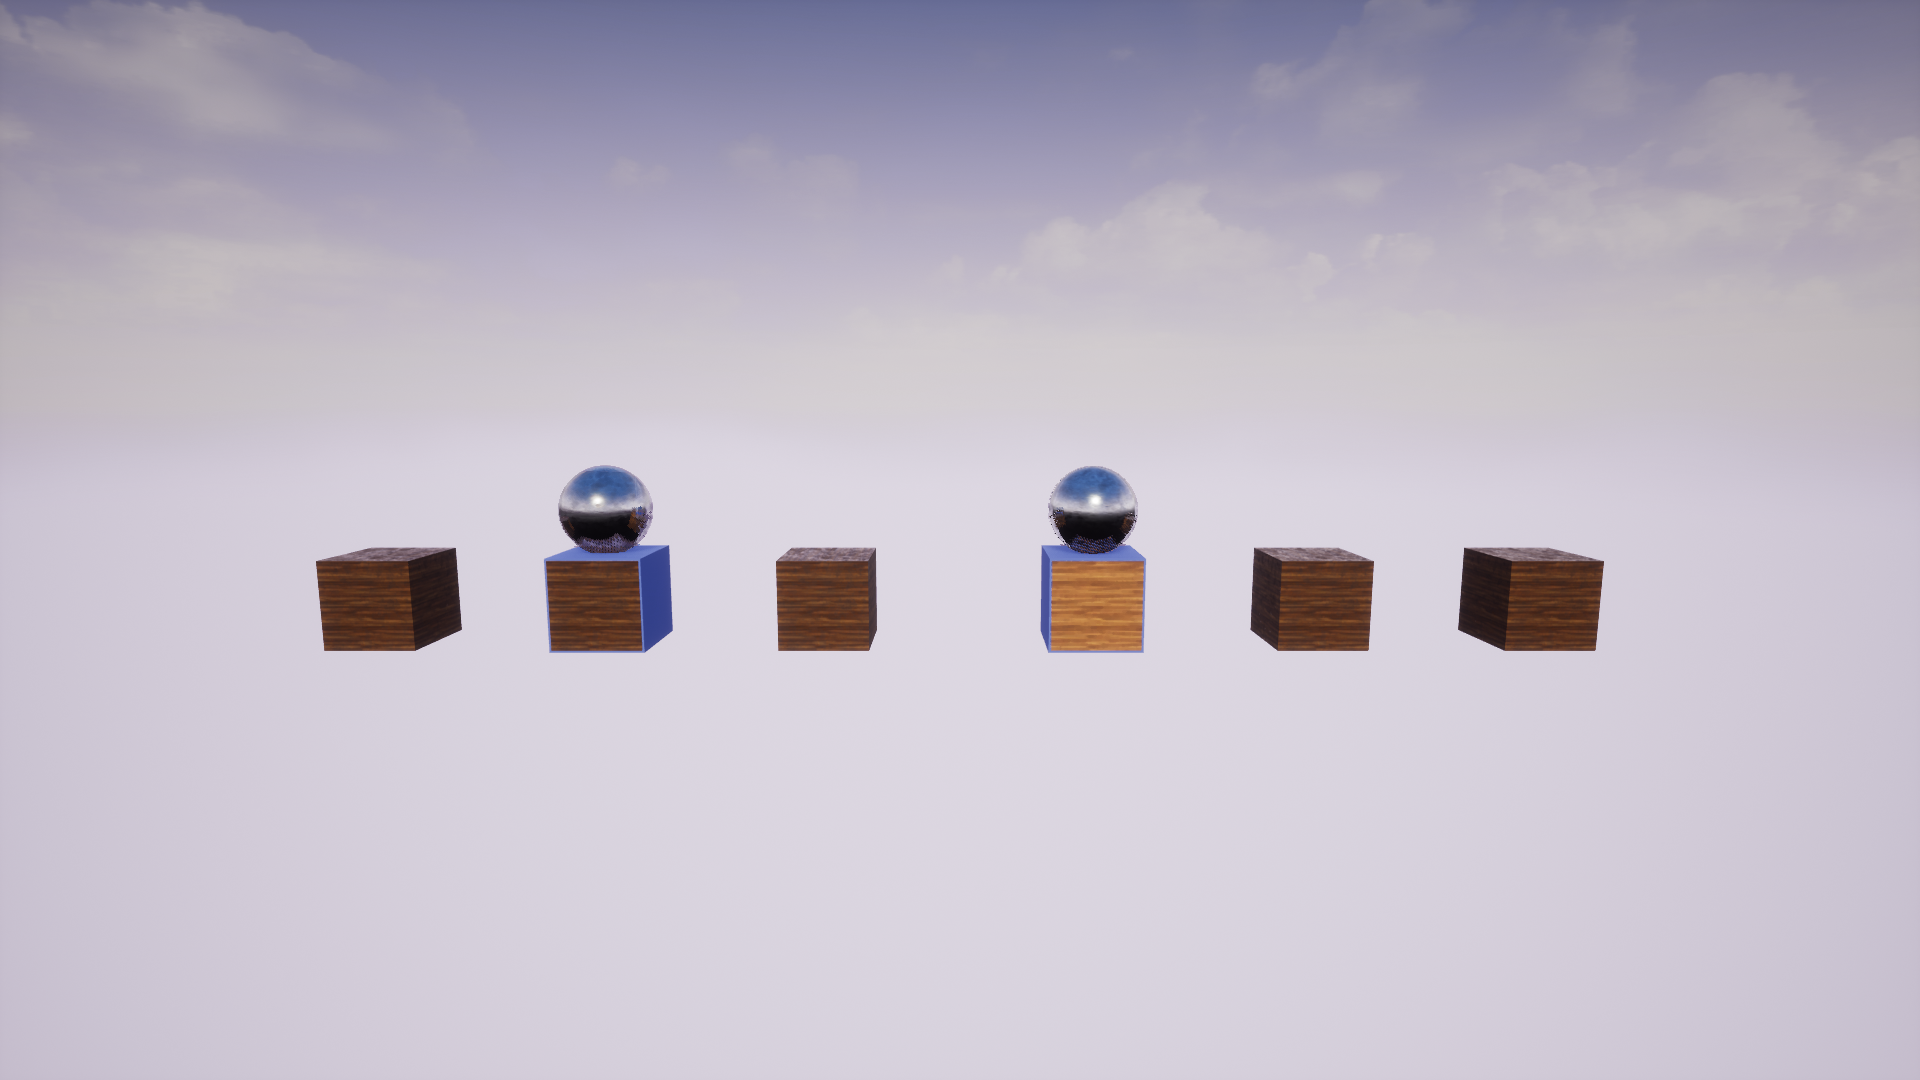
\includegraphics[width=1 \textwidth]{Screenshots/bothStimuli.png}
			\begin{itemize}
				\item The selected boxes blink with changing time offsets
			\end{itemize}
			\begin{itemize}
				\item The Player has determine which side blinked first, choosing his supposed side with the arrow keys.
			\end{itemize}
		\end{posterbox}
		\begin{posterbox}[name=procedure,span=2,column=0,row=2, below=game]{Procedure (game and classical experiment)}
			\begin{center}
				\includegraphics[width=\textwidth, height=100pt]{procedure.png}
			\end{center}
		\end{posterbox}
		
		\begin{posterbox}[name=results,span=1,column=2,row=0]{Analysis}
			\begin{itemize}
				\item The following diagram shows the results of our experiment in a graphical way, by setting the propability to select the first stimulus in relation to the SOA under different delay-parameters. (11 participants)
			\end{itemize}
			\begin{center}
				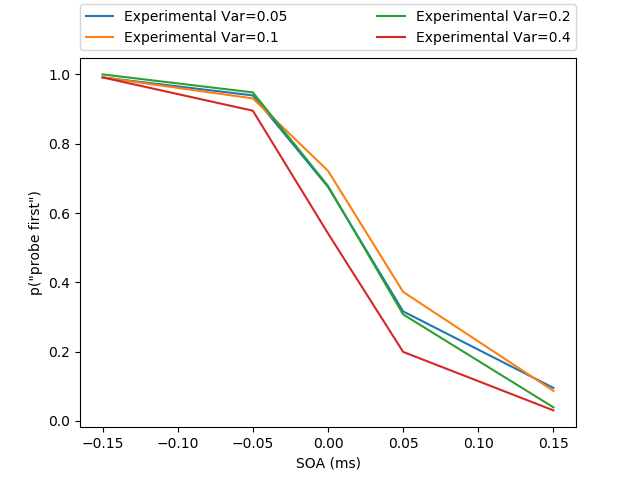
\includegraphics[width=\textwidth]{imgs/complete_data.png}
			\end{center}
			\begin{itemize}
				\item Especially at the SOA of 0ms the difference between the delays is most prominent. 400ms sets itself apart the most.
			\end{itemize}
			
			\begin{center}
				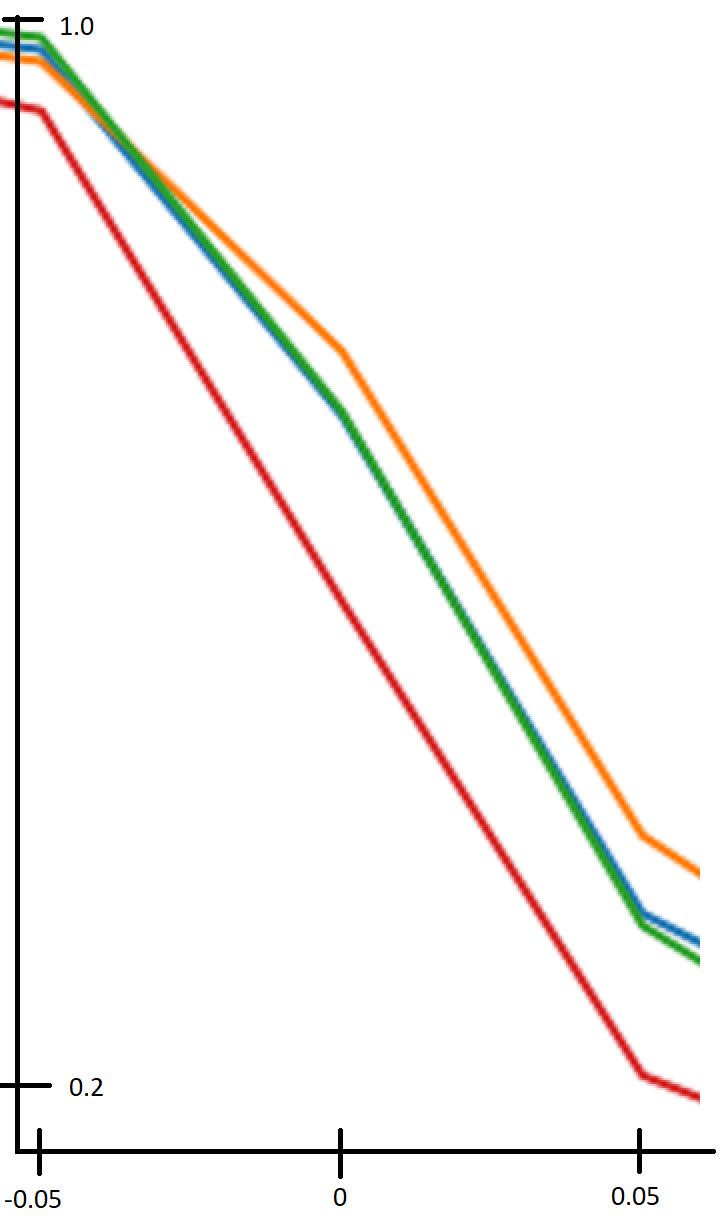
\includegraphics[width=0.7\textwidth]{imgs/data_extract1.png}
			\end{center}
			
			\begin{itemize}
				\item Moreover at SOA 0ms it is clearly visible that time has an effect in our experiment, because the turning-point of the curves are greater than 50 \%
			\end{itemize}
			
		\end{posterbox}
		
		\begin{posterbox}[name=conclusion,span=1,column=2,row=2,below=results]{Conclusion}
			From the results of our experiment, we can derive an effect of time in an temporal order judgement with an colour stimulus.\\
			As expected the time-difference of 400 ms is too large to have a significant impact on the temporal order judgment. On the contrary the delay of 50 ms had a higher impact than expected. Furthermore the delays of 50, 100 and 200 ms only have a small margin of difference even though they have a large impact on the selection of the first stimulus.\\
			To sum up our expectations have been mostly met, but in future work the optimal delay, which seems to be close to 100 ms deducting from our results, should be determined in another experiment .
			\vspace{18pt}
		\end{posterbox}
		
		\begin{posterbox}[name=refs,column=0,span=2,below=procedure,above=bottom]{References}
			\footnotesize
			\linespread{1}
			
			{\color{upbblue}Bundesen, C. } ({\color{upbblue}1998}). A computational theory of visual attention. \textit{Philosophical Transactions of the Royal Society of London B: Biological Sciences, 353, 1271-1281.}, doi: 10.1098/rstb.1998.0282 
			\\\\
			{\color{upbblue}Krüger, A., Tünnermann, J., \& Scharlau, I.} ({\color{upbblue}2016}). Fast and conspicuous? Quantifying salience with the theory of visual attention \textit{Advances in Cognitive Psychology, 12(1), 20}, doi: 10.5709/acp-0184-1
			\\\\
			{\color{upbblue}Dombrowe, I. C., Olivers, C. N. L., \& Donk, M. (2010)} The time course of color- and luminance-based salience effects. Frontiers in Psychology, 1, 189. https://doi.org/10.3389/fpsyg.2010.00189<https://doi.org/10.3389/fpsyg.2010.00189>
			\\\\
			{\color{upbblue}Donk, M., \& Soesman, L. (2011)} Object salience is transiently represented whereas object presence is not: Evidence from temporal order judgment. Perception, 40(1), 63 – 73. https://doi.org/10.1068/p6718 <https://doi.org/10.1068/p6718>
			\\\\
			{\color{upbblue}Wolfe, J. M., \& Horowitz, T. S. (2004)} What attributes guide the deployment of visual attention and how do they do it? Nature Reviews Neuroscience, 5(6), 495–501. https://doi.org/10.1038/nrn1411<https://doi.org/10.1038/nrn1411>
		\end{posterbox}
		
	\end{poster}
\end{document}